\documentclass[semifinal]{cpecmu}
\usepackage{caption}
\usepackage{subcaption}
\usepackage{placeins}


%% This is a sample document demonstrating how to use the CPECMU
%% project template. If you are having trouble, see "cpecmu.pdf" for
%% documentation.

\projectNo{P030-2}
\acadyear{2023}

\titleTH{เเพลตฟอร์มบริหารจัดการโปรเจคแมทชิง}
\titleEN{Project Matching Management Platform}

\author{นายณัฏฐพล ตันจอ}{Nattapon Tancho}{620610786}
\author{นายธิษณ์ธนัย แก้วเพ็ชร์}{Thidtanai Kaewphet}{630610741}

\cpeadvisor{narissara}
\cpecommittee{dome}
\cpecommittee{chinawat}
%%\committee{รศ.ดร.\,นิพนธ์ ธีรอำพน}{Assoc.\,Prof.\,Nipon Theera-Umpon, Ph.D.}

%% Some possible packages to include:
\usepackage[final]{graphicx} % for including graphics

%% Add bookmarks and hyperlinks in the document.
\PassOptionsToPackage{hyphens}{url}
\usepackage[colorlinks=true,allcolors=Blue4,citecolor=red,linktoc=all,breaklinks]{hyperref}
\def\UrlLeft#1\UrlRight{$#1$}

%% Needed just by this example, but maybe not by most reports
\usepackage{afterpage} % for outputting
\usepackage{pdflscape} % for landscape figures and tables. 

%% Some other useful packages. Look these up to find out how to use
%% them.
% \usepackage{natbib}    % for author-year citation styles
% \usepackage{txfonts}
% \usepackage{appendix}  % for appendices on a per-chapter basis
% \usepackage{xtab}      % for tables that go over multiple pages
% \usepackage{subfigure} % for subfigures within a figure
% \usepackage{pstricks,pdftricks} % for access to special PostScript and PDF commands
% \usepackage{nomencl}   % if you have a list of abbreviations

%% if you're having problems with overfull boxes, you may need to increase
%% the tolerance to 9999
\tolerance=9999

\bibliographystyle{plain}
% \bibliographystyle{IEEEbib}

% \renewcommand{\topfraction}{0.85}
% \renewcommand{\textfraction}{0.1}
% \renewcommand{\floatpagefraction}{0.75}

%% Example for glossary entry
%% Need to use glossary option
%% See glossaries package for complete documentation.
\ifglossary
  \newglossaryentry{lorem ipsum}{
    name=lorem ipsum,
    description={derived from Latin dolorem ipsum, translated as ``pain itself''}
  }
\fi

%% Uncomment this command to preview only specified LaTeX file(s)
%% imported with \include command below.
%% Any other file imported via \include but not specified here will not
%% be previewed.
%% Useful if your report is large, as you might not want to build
%% the entire file when editing a certain part of your report.
%\includeonly{chapters/background}

\begin{document}
\maketitle
\makesignature

\ifproject
\begin{abstractTH}
    \hspace{4ex} 
    โครงงานนี้จัดทำขึ้นเพื่อพัฒนาระบบที่จะช่วยเพิ่มช่องทางและประสบการณ์ในการประกาศและเข้าร่วมกิจกรรมในมหาวิทยาลัยเชียงใหม่ผ่านเว็บแอปพลิเคชัน
    โดยเราจะมีระบบการสร้างและเข้าร่วมกิจกรรม รวมถึงมีระบบแนะนํากิจกรรมเพื่อใช้ในการแนะนํากิจกรรมที่เหมาะสมกับความสนใจของผู้ใช้
\end{abstractTH}

\begin{abstract}
    \hspace{4ex} 
    This project is undertaken to develop a system that will enhance avenues and experiences for announcing and participating in activities within Chiang Mai University through a web application. We will have systems for creating and joining activities, as well as a recommendation system to suggest activities suitable for users based on their interests.

\end{abstract}

\iffalse
\begin{dedication}
This document is dedicated to all Chiang Mai University students.

Dedication page is optional.
\end{dedication}
\fi % \iffalse

\begin{acknowledgments}
    \hspace{4ex} โครงงานนี้สำเร็จลุล่วงได้ด้วยความกรุณาจาก รศ.ดร.นริศรา เอี่ยมคณิตชาติ อาจารย์ที่ปรึกษาผู้ซึ่งได้สละเวลาให้ความช่วยเหลือ ทั้งในการให้ความรู้ คำแนะนำ รวมทั้งแนะแนวทางการดำเนินงาน จนทำให้โครงงานนี้สำเร็จลุล่วงไปได้

    \enskip ขอขอบพระคุณ ผศ.โดม โพธิกานนท์ และ อ.ดร.ชินวัตร อิศราดิสัยกุล อาจารย์กรรมการ ที่ได้ให้คำแนะนำต่างๆ ซึ่งทำให้โครงงานนี้มีความสมบูรณ์และพัฒนาไปได้อย่างตรงตามวัตถุประสงค์มากยิ่งขึ้น

    \enskip หากโครงงานนี้มีข้อบกพร่องประการใด ผู้จัดทำต้องขออภัยเป็นอย่างสูง
% \texttt{acknowledgment}

\acksign{2024}{3}{29}
\end{acknowledgments}%
\fi % \ifproject

\contentspage

\ifproject
\figurelistpage

\tablelistpage
\fi % \ifproject

% \abbrlist % this page is optional

% \symlist % this page is optional

% \preface % this section is optional


\pagestyle{empty}\cleardoublepage
\normalspacing \setcounter{page}{1} \pagenumbering{arabic} \pagestyle{cpecmu}

\include{chapters/intro}
\include{chapters/background}
\chapter{\ifproject%
\ifenglish Project Structure and Methodology\else โครงสร้างและขั้นตอนการทำงาน\fi
\else%
\ifenglish Project Structure\else โครงสร้างของโครงงาน\fi
\fi
}

% ในบทนี้จะกล่าวถึงหลักการ และการออกแบบระบบ

\makeatletter

% \renewcommand\section{\@startsection {section}{1}{\z@}%
%                                    {13.5ex \@plus -1ex \@minus -.2ex}%
%                                    {2.3ex \@plus.2ex}%
%                                    {\normalfont\large\bfseries}}

\makeatother
%\vspace{2ex}
% \titleformat{\section}{\normalfont\bfseries}{\thesection}{1em}{}
% \titlespacing*{\section}{0pt}{10ex}{0pt}



\section{หลักการทำงานของแอปพลิเคชัน}
โครงงานนี้เป็นแอปพลิเคชันที่ช่วยในการสร้าง, ประกาศกิจกรรม และเข้าร่วมกิจกรรมของนักศึกษาและบุคลากรของมหาวิทยาลัยเชียงใหม่ที่มี CMU-Account
โดยเลือกพัฒนาเป็นเว็บแอปพลิเคชัน มีระบบที่ให้ผู้ใช้สร้างและประชาสัมพันธ์กิจกรรม, ดูข้อมูลและขอเข้าร่วมกิจกรรมที่ตนเองสนใจ โดยทางเว็บจะมีระบบแนะนำกิจกรรมที่ตรงกับความสนใจของผู้ใช้มากที่สุด และยังมีการนำสถิติการใช้งานเว็บแอปพลิเคชันในส่วนต่างๆมาวิเคราะห์และนำเสนอในรูปแบบที่เข้าใจง่าย โดยใช้ความรู้ด้าน Data Visualization
\begin{figure}[h] %h = here. other are top,bottom,separate page(p)
\begin{center}
\includegraphics[width=0.9\linewidth]{image/31_system_overview.png}
\end{center}
\caption[Poem]{System Overview}
\label{fig:system_overview}
\end{figure}
\section{การใช้งานแอปพลิเคชัน}
เว็บแอปพลิเคชันนี้จะแบ่งกลุ่มผู้ใช้ออกเป็น 2 กลุ่ม ได้แก่
\subsection{ผู้ใช้ทั่วไป}
สิ่งที่ผู้ใช้ทั่วไปสามารถใช้งานได้ ได้แก่
\begin{itemize}
    \item สามารถค้นหากิจกรรมได้ ทั้งจากการพิมพ์คำสำคัญ ในช่องค้นหา และหน้าข่าวสารกิจกรรมทั้งหมด
    \item สามารถดูรายละเอียดของแต่ละกิจกรรมได้
    \item อ่านความคิดเห็นของแต่ละกิจกรรมได้
    \item ติดต่อสอบถาม หรือส่งข้อเสนอแนะเกี่ยวกับเว็บแอปพลิเคชันได้
\end{itemize}
\subsection{ผู้ใช้ที่ยืนยันตัวตนด้วย CMU-OAuth}
หลังจากผู้ใช้ลงทะเบียนเข้าใช้งานด้วย CMU Account แล้ว สิ่งที่ผู้ใช้สามารถทำได้เพิ่มมากขึ้น ได้แก่
\begin{itemize}
    \item สามารถตั้งชื่อ username เพื่อใช้เป็นนามแฝงได้
    \item สร้างกิจกรรมใหม่ขึ้นมา ทั้งแบบต้องการสมาชิกหรือแค่ประชาสัมพันธ์กิจกรรม
    \item แสดงความคิดเห็นในแต่ละหน้ากิจกรรมได้
    \item สามารถสมัครเข้าร่วมกิจกรรมที่สนใจได้
    \item สามารถดูปฏิทินเพื่อตรวจสอบวัน/เวลาแต่ละกิจกรรมได้
    \item สามารถเข้าหน้า Dashboard เพื่อดูข้อมูลสถิติของเว็บได้
\end{itemize}
\section{นโยบายความเป็นส่วนตัว}
เมื่อผู้ใช้ลงชื่อเข้าใช้งานครั้งแรก ผู้ใช้จะต้องตั้งค่า username เพื่อใช้เป็นนามแฝงในการแสดงความคิดเห็นในหน้ากิจกรรม

\section{การออกแบบหน้าเว็บแอปพลิเคชัน}
ในการออกแบบหน้าเว็บแอปพลิชัน พวกเราได้เลือกใช้ Figma เพราะเป็นเครื่องมือที่อำนวยความสะดวก ในการออกแบบหน้าเว็บแอปพลิเคชัน ช่วยให้การออกแบบ UI/UX สะดวกมากขึ้น อีกทั้งยังเป็นเครื่องมือที่ผู้คนต่างก็นิยมใช้
ทำให้ผู้ใช้ทั่วโลกสามารถแชร์วิธีการออกแบบ ทำให้สามารถนำไปเป็นไอเดียในการออกแบบได้ 
\begin{figure}[h]
  \centering
  \begin{subfigure}[b]{0.4\linewidth}
    \includegraphics[width=\linewidth]{image/Figma-design/Main-not-login.png}
    \caption{แสดงข้อมูลของเว็บ}
  \end{subfigure}
  \hfill
  \begin{subfigure}[b]{0.4\linewidth}
    \includegraphics[width=\linewidth]{image/Figma-design/Main-recomendation.png}
    \caption{แสดงแบบสอบถามกิจกรรมที่สนใจ}
  \end{subfigure}
  \caption{หน้าแรก}
  \label{fig:main}
\end{figure}

\begin{figure}[h]
  \centering
  \begin{subfigure}[b]{0.3\linewidth}
    \includegraphics[width=\linewidth]{image/Figma-design/New-Event-info.png}
    \caption{แสดงรายการกิจกรรมต่างๆ}
  \end{subfigure}
  \hfill
  \begin{subfigure}[b]{0.3\linewidth}
    \includegraphics[width=\linewidth]{image/Figma-design/New-Event-info2.png}
    \caption{แสดงรายละเอียดของกิจกรรม}
  \end{subfigure}
  \caption{หน้ารายการกิจกรรม}
  \label{fig:event-info}
\end{figure}

\begin{figure}[h]
  \centering
  \begin{subfigure}[b]{0.3\linewidth}
    \includegraphics[width=\linewidth]{image/Figma-design/New-Event-join.png}
    \caption{แสดงหน้าคำขอเข้าร่วม}
  \end{subfigure}
  \hfill
  \begin{subfigure}[b]{0.3\linewidth}
    \includegraphics[width=\linewidth]{image/Figma-design/New-Event-join-noti.png}
    \caption{แสดงรายการคำขอเข้าร่วม}
  \end{subfigure}
  \caption{หน้าการขอเข้าร่วมกิจกรรม}
  \label{fig:event-join}
\end{figure}

\begin{figure}[h]
  \centering
  \begin{subfigure}[b]{0.3\linewidth}
    \includegraphics[width=\linewidth]{image/Figma-design/Create-event-info.png}
    \caption{กรอกข้อมูลสร้างกิจกรรม}
  \end{subfigure}
  \hfill
  \begin{subfigure}[b]{0.3\linewidth}
    \includegraphics[width=\linewidth]{image/Figma-design/Create-event-info-1.png}
    \caption{แสดงข้อความสร้างสำเร็จ}
  \end{subfigure}
  \caption{หน้าสร้างกิจกรรม}
  \label{fig:event-create}
\end{figure}

\begin{figure}[h]
  \centering
  \begin{subfigure}[b]{0.3\linewidth}
    \includegraphics[width=\linewidth]{image/Figma-design/New-Mine-event.png}
    \caption{แสดงกิจกรรมที่เข้าร่วมอยู่}
  \end{subfigure}
  \hfill
  \begin{subfigure}[b]{0.3\linewidth}
    \includegraphics[width=\linewidth]{image/Figma-design/New-Mine-event2.png}
    \caption{แสดงรายละเอียดกิจกรรมที่เข้าร่วมอยู่}
  \end{subfigure}
  \caption{หน้ารายการกิจกรรมที่เข้าร่วม}
  \label{fig:event-mine}
\end{figure}

\begin{figure}[h]
  \centering
  \begin{subfigure}[b]{0.3\linewidth}
    \includegraphics[width=\linewidth]{image/Figma-design/mobile-main.png}
    \caption{แสดงหน้าแรก}
  \end{subfigure}
  \hfill
  \begin{subfigure}[b]{0.3\linewidth}
    \includegraphics[width=\linewidth]{image/Figma-design/mobile-recomendation.png}
    \caption{แสดงแบบสอบถามความสนใจ}
  \end{subfigure}
  \caption{หน้าการแสดงผลในโทรศัพท์}
  \label{fig:mobile}
\end{figure}

\FloatBarrier

\section{โครงสร้างการไหลของข้อมูล}
โครงสร้างการไหลของข้อมูลแบ่งออกเป็น 3 ส่วน ได้แก่ User, System และ Admin
โดยข้อมูลที่userจะส่งไปให้ system ได้แก่ ข้อมูลของผู้ใช้,ข้อมูลการกดสนใจเข้าร่วมกิจกรรม,คำขอเข้าร่วมกิจกรรม,คำขอสร้างกิจกรรม
จากนั้น system จะส่งข้อมูลคำขอสร้างกิจกรรมไปให้ admin ในการอนุมัติ แล้วจึงจะส่งผลการอนุมัติไปพร้อมกับข้อมูลที่จะแสดงผลไปให้ user
ซึ่ง user ที่เป็นผู้สร้างกิจกรรมที่ได้รับคำขอเข้าร่วมกิจกรรม จะสามารถส่งผลการขอเข้าร่วมไปให้ system แล้วส่งต่อให้ user ที่ขอต่อไป ตามดังในรูปภาพที่3.7
\begin{figure}[h]
\begin{center}
\includegraphics[width=0.9\linewidth]{image/dataflow-diagram.png}
\end{center}
\caption[Poem]{แผนผังการไหลของข้อมูล}
\label{fig:dataflow}
\end{figure}
% \subsection{The Black Kitten}
%   One thing was certain, that the WHITE kitten had had nothing to
% do with it:---it was the black kitten's fault entirely~\cite{aiw}.  For the
% white kitten had been having its face washed by the old cat for
% the last quarter of an hour (and bearing it pretty well,
% considering); so you see that it COULDN'T have had any hand in
% the mischief.

%   The way Dinah washed her children's faces was this:  first she
% held the poor thing down by its ear with one paw, and then with
% the other paw she rubbed its face all over, the wrong way,
% beginning at the nose:  and just now, as I said, she was hard at
% work on the white kitten, which was lying quite still and trying
% to purr---no doubt feeling that it was all meant for its good.

%   But the black kitten had been finished with earlier in the
% afternoon, and so, while Alice was sitting curled up in a corner
% of the great arm-chair, half talking to herself and half asleep,
% the kitten had been having a grand game of romps with the ball of
% worsted Alice had been trying to wind up, and had been rolling it
% up and down till it had all come undone again; and there it was,
% spread over the hearth-rug, all knots and tangles, with the
% kitten running after its own tail in the middle.

% \subsection{The Reproach}

%   `Oh, you wicked little thing!' cried Alice, catching up the
% kitten, and giving it a little kiss to make it understand that it
% was in disgrace.  `Really, Dinah ought to have taught you better
% manners!  You OUGHT, Dinah, you know you ought!' she added,
% looking reproachfully at the old cat, and speaking in as cross a
% voice as she could manage---and then she scrambled back into the
% arm-chair, taking the kitten and the worsted with her, and began
% winding up the ball again.  But she didn't get on very fast, as
% she was talking all the time, sometimes to the kitten, and
% sometimes to herself.  Kitty sat very demurely on her knee,
% pretending to watch the progress of the winding, and now and then
% putting out one paw and gently touching the ball, as if it would
% be glad to help, if it might.

%   `Do you know what to-morrow is, Kitty?' Alice began.  `You'd
% have guessed if you'd been up in the window with me---only Dinah
% was making you tidy, so you couldn't.  I was watching the boys
% getting in stick for the bonfire---and it wants plenty of
% sticks, Kitty!  Only it got so cold, and it snowed so, they had
% to leave off.  Never mind, Kitty, we'll go and see the bonfire
% to-morrow.'  Here Alice wound two or three turns of the worsted
% round the kitten's neck, just to see how it would look:  this led
% to a scramble, in which the ball rolled down upon the floor, and
% yards and yards of it got unwound again.

%   `Do you know, I was so angry, Kitty,' Alice went on as soon as
% they were comfortably settled again, `when I saw all the mischief
% you had been doing, I was very nearly opening the window, and
% putting you out into the snow!  And you'd have deserved it, you
% little mischievous darling!  What have you got to say for
% yourself?  Now don't interrupt me!' she went on, holding up one
% finger.  `I'm going to tell you all your faults.  Number one:
% you squeaked twice while Dinah was washing your face this
% morning.  Now you can't deny it, Kitty:  I heard you!  What that
% you say?' (pretending that the kitten was speaking.)  `Her paw
% went into your eye?  Well, that's YOUR fault, for keeping your
% eyes open---if you'd shut them tight up, it wouldn't have
% happened.  Now don't make any more excuses, but listen!  Number
% two:  you pulled Snowdrop away by the tail just as I had put down
% the saucer of milk before her!  What, you were thirsty, were you?

\ifproject
\chapter{\ifproject%
\ifenglish Experimentation and Results\else การทดลองและผลลัพธ์\fi
\else%
\ifenglish System Evaluation\else การประเมินระบบ\fi
\fi}

\hspace{4ex} 
ในบทนี้จะกล่าวถึงผลการทดสอบการทำงานของเว็บแอปพลิเคชัน โดยจะทำการทดสอบผ่านหน้าเว็บแอปพลิเคชัน

\section{ผลการทดสอบการทำงานของหน้าเว็บ}
ผลการทำงานต่างๆที่ทดสอบจากหน้าเว็บแอปพลิเคชัน
\subsection{ระบบการลงทะเบียนและการเข้าสู่ระบบ}
ผู้ใช้สามารถลงทะเบียนและเข้าสู่ระบบได้
\begin{figure}[h]
  \centering
  \begin{subfigure}[b]{0.4\linewidth}
    \includegraphics[width=\linewidth]{image/web/register.jpeg}
    \caption{หน้าล็อกลงทะเบียน}
  \end{subfigure}
  \hfill
  \begin{subfigure}[b]{0.4\linewidth}
    \includegraphics[width=\linewidth]{image/web/login.jpeg}
    \caption{หน้าเข้าสู่ระบบ}
  \end{subfigure}
  \caption{ผลการลงทะเบียนและการเข้าสู่ระบบ}
  \label{fig:register-login}
\end{figure}

\subsection{ระบบเลือกความสนใจ}
มีหน้าเลือกความสนใจแสดงขึ้นมาให้ผู้ใช้หากผู้ใช้เข้าสู่ระบบเป็นครั้งแรก
\begin{figure}[h] 
    \begin{center}
        \includegraphics[width=0.6\linewidth]{image/web/choose.jpeg}
    \end{center}
    \caption{ผลการแสดงหน้าเลือกความสนใจหลังเข้าสู่ระบบครั้งแรก}
    \label{fig:choose}
\end{figure}

\newpage

\subsection{การแสดงผลระหว่างผู้ใช้ที่เข้าสู่ระบบแล้วกับยังไม่ได้เข้าสู่ระบบ}
ผู้ใช้ที่ไม่ได้เข้าสู่ระบบจะสามารถดูได้แค่หน้าหลักและหน้าข่าวสารกิจกรรม ส่วนผู้ใช้ที่เข้าสู่ระบบแล้วจะสามารถเข้าถึงหน้าต่างๆได้เพิ่มขึ้น
\begin{figure}[h]
  \centering
  \begin{subfigure}[b]{0.4\linewidth}
    \includegraphics[width=\linewidth]{image/web/notLog-activity.jpeg}
    \caption{หน้าข่าวสารกิจกรรมของผู้ใช้ที่ยังไม่ได้เข้าสู่ระบบ}
  \end{subfigure}
  \hfill
  \begin{subfigure}[b]{0.4\linewidth}
    \includegraphics[width=\linewidth]{image/web/activity.jpeg}
    \caption{หน้าข่าวสารกิจกรรมของผู้ใช้ที่เข้าสู่ระบบแล้ว}
  \end{subfigure}
  \caption{ผลการแสดงผลระหว่างผู้ใช้ที่เข้าสู่ระบบแล้วกับยังไม่ได้เข้าสู่ระบบ}
  \label{fig:loginShow}
\end{figure}

\FloatBarrier

\newpage
\subsection{ระบบแนะนำกิจกรรมที่ผู้ใช้อาจสนใจ}
หลังจากที่ผู้ใช้เลือกแท็กกิจกรรมที่สนใจแล้วจะมีส่วนของกิจกรรมที่แนะนำแสดงเพิ่มขึ้นมา โดยกิจกรรมที่แนะนำนั้นจะตรงกับแท็กที่ผู้ใช้เลือก
\begin{figure}[h]
  \centering
  \begin{subfigure}[b]{0.4\linewidth}
    \includegraphics[width=\linewidth]{image/web/choose.jpeg}
    \caption{แท็กกิจกรรมที่ผู้ใช้เลือก}
  \end{subfigure}
  \hfill
  \begin{subfigure}[b]{0.4\linewidth}
    \includegraphics[width=\linewidth]{image/web/recommend.jpg}
    \caption{กิจกรรมที่แนะนำให้กับผู้ใช้}
  \end{subfigure}
  \caption{ผลแนะนำกิจกรรมที่ผู้ใช้อาจสนใจ}
  \label{fig:reccomended}
\end{figure}

\FloatBarrier

\subsection{ระบบประกาศกิจกรรม}
ผู้ใช้สามารถสร้างกิจกรรมขึ้นมาใหม่ได้ และสามารถเลือกได้ว่าจะเปิดรับสมัครตำแหน่งอะไรด้วยไหมได้ โดยหลังจากสร้างกิจกรรมแล้ว กิจกรรมนั้นจะถูกประกาศในหน้าประกาศกิจกรรมโดยมีข้อมูลแสดงถูกต้อง
\begin{figure}[h]
  \centering
  \begin{subfigure}[b]{0.4\linewidth}
    \includegraphics[width=\linewidth]{image/web/create.jpeg}
    \caption{หน้าสร้างกิจกรรม}
  \end{subfigure}
  \hfill
  \begin{subfigure}[b]{0.4\linewidth}
    \includegraphics[width=\linewidth]{image/web/showCreate.jpg}
    \caption{กิจกรรมถูกประกาศหลังจากที่ถูกสร้างแล้ว}
  \end{subfigure}
  \caption{ผลการประกาศกิจกรรม}
  \label{fig:create}
\end{figure}

\FloatBarrier

\subsection{ระบบกิจกรรมของฉัน}
หลังจากที่ผู้ใช้กดสนใจกิจกรรมหรือสมัครเข้าร่วมกิจกรรมใดๆ กิจกรรมนั้นๆจะถูกแสดงในหน้ากิจกรรมของฉัน
\begin{figure}[h]
  \centering
  \begin{subfigure}[b]{0.4\linewidth}
    \includegraphics[width=\linewidth]{image/web/showInfo.jpg}
    \caption{กดสนใจกิจกรรม}
  \end{subfigure}
  \hfill
  \begin{subfigure}[b]{0.4\linewidth}
    \includegraphics[width=\linewidth]{image/web/myAct.jpeg}
    \caption{กิจกรรมถูกแสดงในหน้ากิจกรรมของฉัน}
  \end{subfigure}
  \caption{ผลการกดสนใจกิจกรรม}
  \label{fig:interests}
\end{figure}

\FloatBarrier

\subsection{ระบบสมัครตำแหน่งในกิจกรรม}
หลังจากที่ผู้ใช้กดสมัครกิจกรรมในตำแหน่งที่สนใจไป จะมีหน้าต่างให้กรอกคำขอสมัคร หลังจากกดส่งคำขอสมัครแล้ว คำขอจะส่งถูกส่งไปยังผู้สร้างกิจกรรมนั้นๆโดยผู้ใช้จะสามารถดูคำขอต่างๆได้จากปุ่มกระดิ่งแจ้งเตือน อีกทั้งยังสามารถตอบรับหรือปฏิเสธคำขอได้
\begin{figure}[h]
  \centering
  \begin{subfigure}[b]{0.4\linewidth}
    \includegraphics[width=\linewidth]{image/web/createReq.jpg}
    \caption{ผู้ใช้กรอกข้อมูลสมัครตำแหน่งของกิจกรรมไป}
  \end{subfigure}
  \hfill
  \begin{subfigure}[b]{0.4\linewidth}
    \includegraphics[width=\linewidth]{image/web/joinReq.jpg}
    \caption{ผู้สร้างกิจกรรมเห็นคำขอสมัครเข้าร่วม}
  \end{subfigure}
  \caption{ผลระบบสมัครตำแหน่งในกิจกรรม}
  \label{fig:joinReq}
\end{figure}

\FloatBarrier
\chapter{\ifenglish Conclusions and Discussions\else บทสรุปและข้อเสนอแนะ\fi}

\section{\ifenglish Conclusions\else สรุปผล\fi}

\hspace{4ex} 
จากการพัฒนาโครงงาน Project Matching Management Platform ระบบที่ได้ สามารถทำงานได้ตามวัตถุประสงค์ของโครงงานซึ่งก็คือสามารถพัฒนาเว็บแอปพลิเคชันที่สามารถรองรับการประกาศกิจกรรมและเข้าร่วมกิจกรรมได้อย่างถูกต้อง อีกทั้งสามารถพัฒนาระบบที่สามารถนำข้อมูลของผู้ใช้มาใช้ในการแนะนำกิจกรรมให้กับผู้ใช้ได้

\section{\ifenglish Challenges\else ปัญหาที่พบและแนวทางการแก้ไข\fi}

ในการทำโครงงานนี้ พบว่าเกิดปัญหาหลักๆ ดังนี้
\begin{enumerate}
    \item การพูดคุยระหว่างผู้พัฒนามีจำนวนน้อยเกินไปทำให้งานดำเนินไปได้ด้วยความล่าช้า และทำให้เกิดปัญหาในการดำเนินงาน
    \item ไม่สามารถหาข้อมูลสถิติการเข้าร่วมกิจกรรมต่างๆของนักศึกษาแบ่งตามแท็กกิจกรรมได้ ทำให้ระบบแนะนำกิจกรรมที่ได้มีประสิทธิภาพไม่เป็นอย่างที่ออกแบบไว้
    \item คิดออกแบบโครงงานได้ไม่ดีเพียงพอ ทำให้ตอนพัฒนาจริงต้องปรับเปลี่ยนอะไรต่างๆจากที่ออกแบบไว้มากกว่าที่ควร
    \item วางแผนเวลาการดำเนินงานได้ไม่ดีพอ และ ใช้เวลาในการคิดออกแบบระบบต่างๆมากเกินไป แล้วไม่ได้ลงมือปฏิบัติจริงซักที ทำให้เวลาในการพัฒนาไม่เพียงพอ
\end{enumerate}

\section{\ifenglish%
Suggestions and further improvements
\else%
ข้อเสนอแนะและแนวทางการพัฒนาต่อ
\fi
}

ข้อเสนอแนะเพื่อพัฒนาโครงงานนี้ต่อไป มีดังนี้

\begin{enumerate}
    \item พัฒนาระบบแนะนำจากการนำข้อมูลของแท็กของผู้ใช้ไปทำการเสิร์ช เป็นการนำข้อมูลต่างๆของผู้ใช้ไปทำการประมวลผลหาแนวโน้มร่วมกับผู้ใช้อื่นๆด้วย
    \item จัดการเคลียร์โค้ดใหม่ให้มีประสิทธิภาพมากยิ่งขึ้น 
    \item พัฒนาระบบให้สามารถใช้กับ CMU Account ได้
    \item เพิ่มระบบการจัดการสมาชิกในกิจกรรม
    \item เพิ่มระบบรีวิวกิจกรรม
    \item เพิ่มการทำงานฝั่ง Admin
    \item เพิ่มระบบสรุปผลการเข้าร่วมกิจกรรมของผู้ใช้
    \item นำเว็บแอปพลิเคชันไป deploy บน Cloud
\end{enumerate}

\fi

\bibliography{sampleReport}

\ifproject
\normalspacing
\appendix
\include{chapters/appendix}

%% Display glossary (optional) -- need glossary option.
\ifglossary\glossarypage\fi

%% Display index (optional) -- need idx option.
\ifindex\indexpage\fi

\begin{biosketch}
\begin{center}
  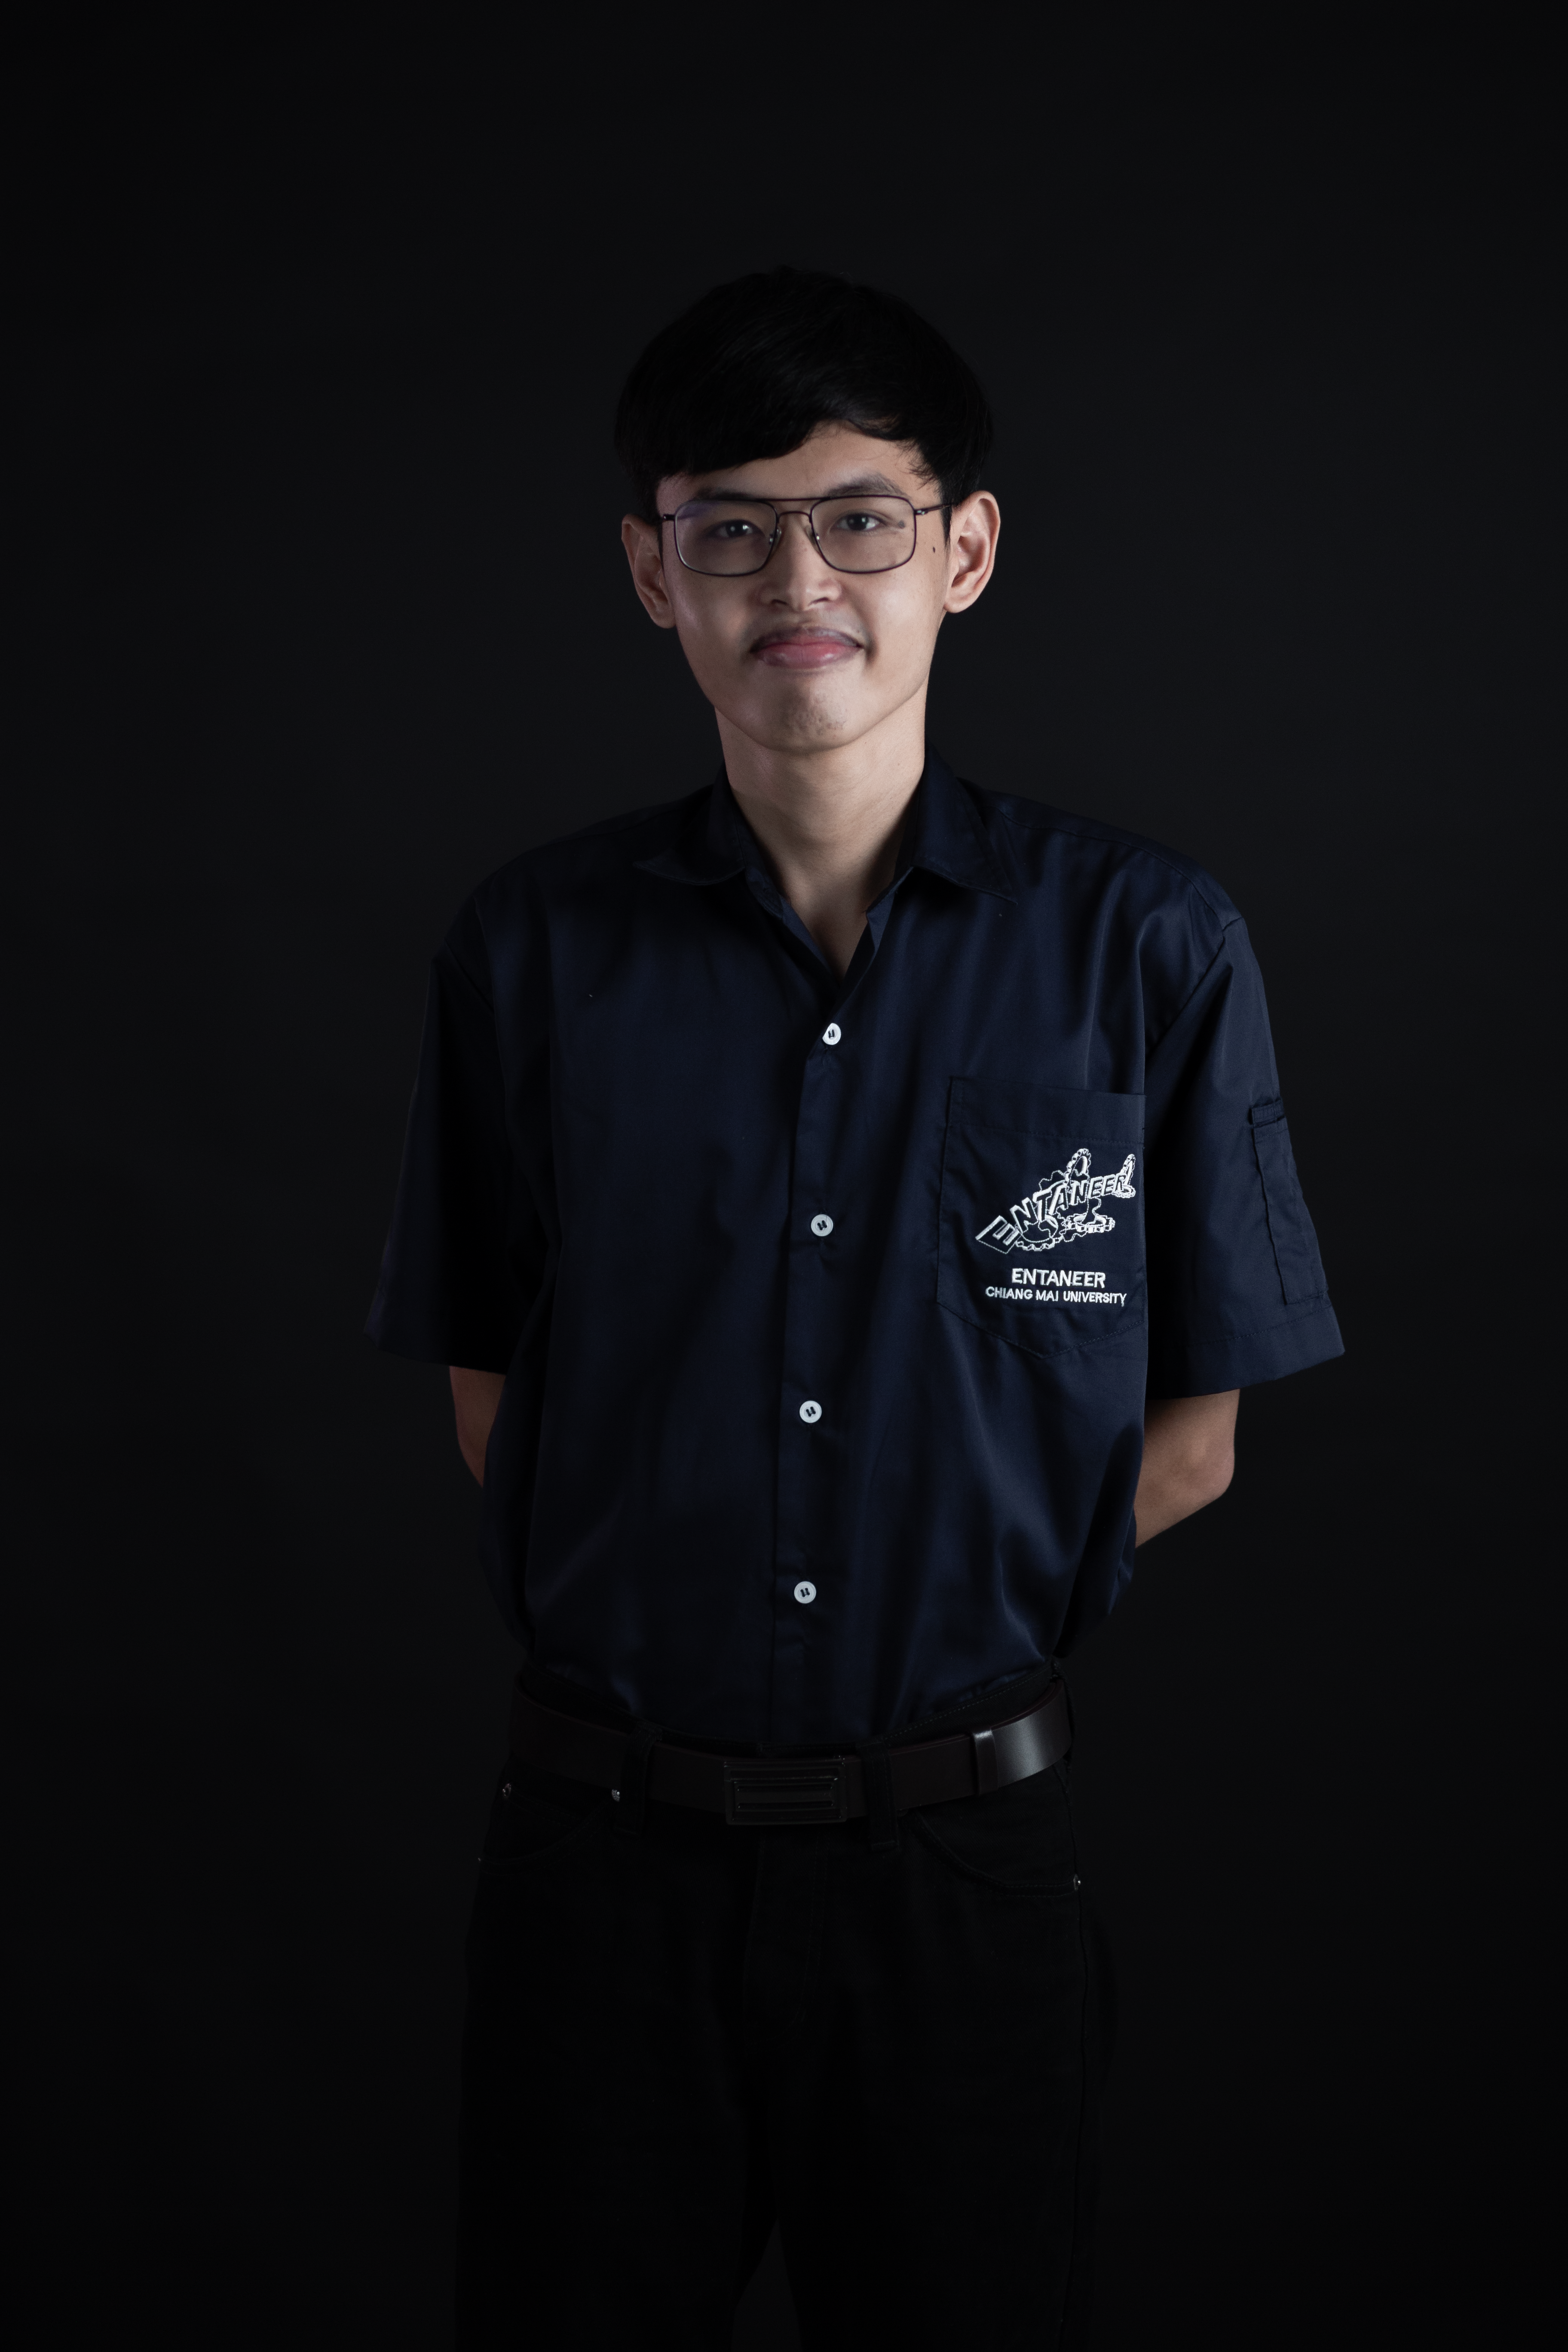
\includegraphics[width=1.5in]{image/boy_shop_uniform.png}
\end{center}
นายณัฏฐพล ตันจอ เกิดเมื่อวันที่ 28 ตุลาคม พศ.2540 ณ จังหวัดสระบุรี สําเร็จการศึกษาระดับ
มัธยมปลาย จาก กำแพงเพชรพิทยาคม จังหวัดกำแพงเพชร เข้าศึกษาที่คณะวิศวกรรมศาสตร์ สาขาวิศวกรรมคอมพิวเตอร์ มหาวิทยาลัยเชียงใหม่ เมื่อเดือนสิงหาคม พ.ศ.2562 มีประสปการณ์ พัฒนาเว็บแอปพลิเคชัน, network design, cloud service
\begin{center}
  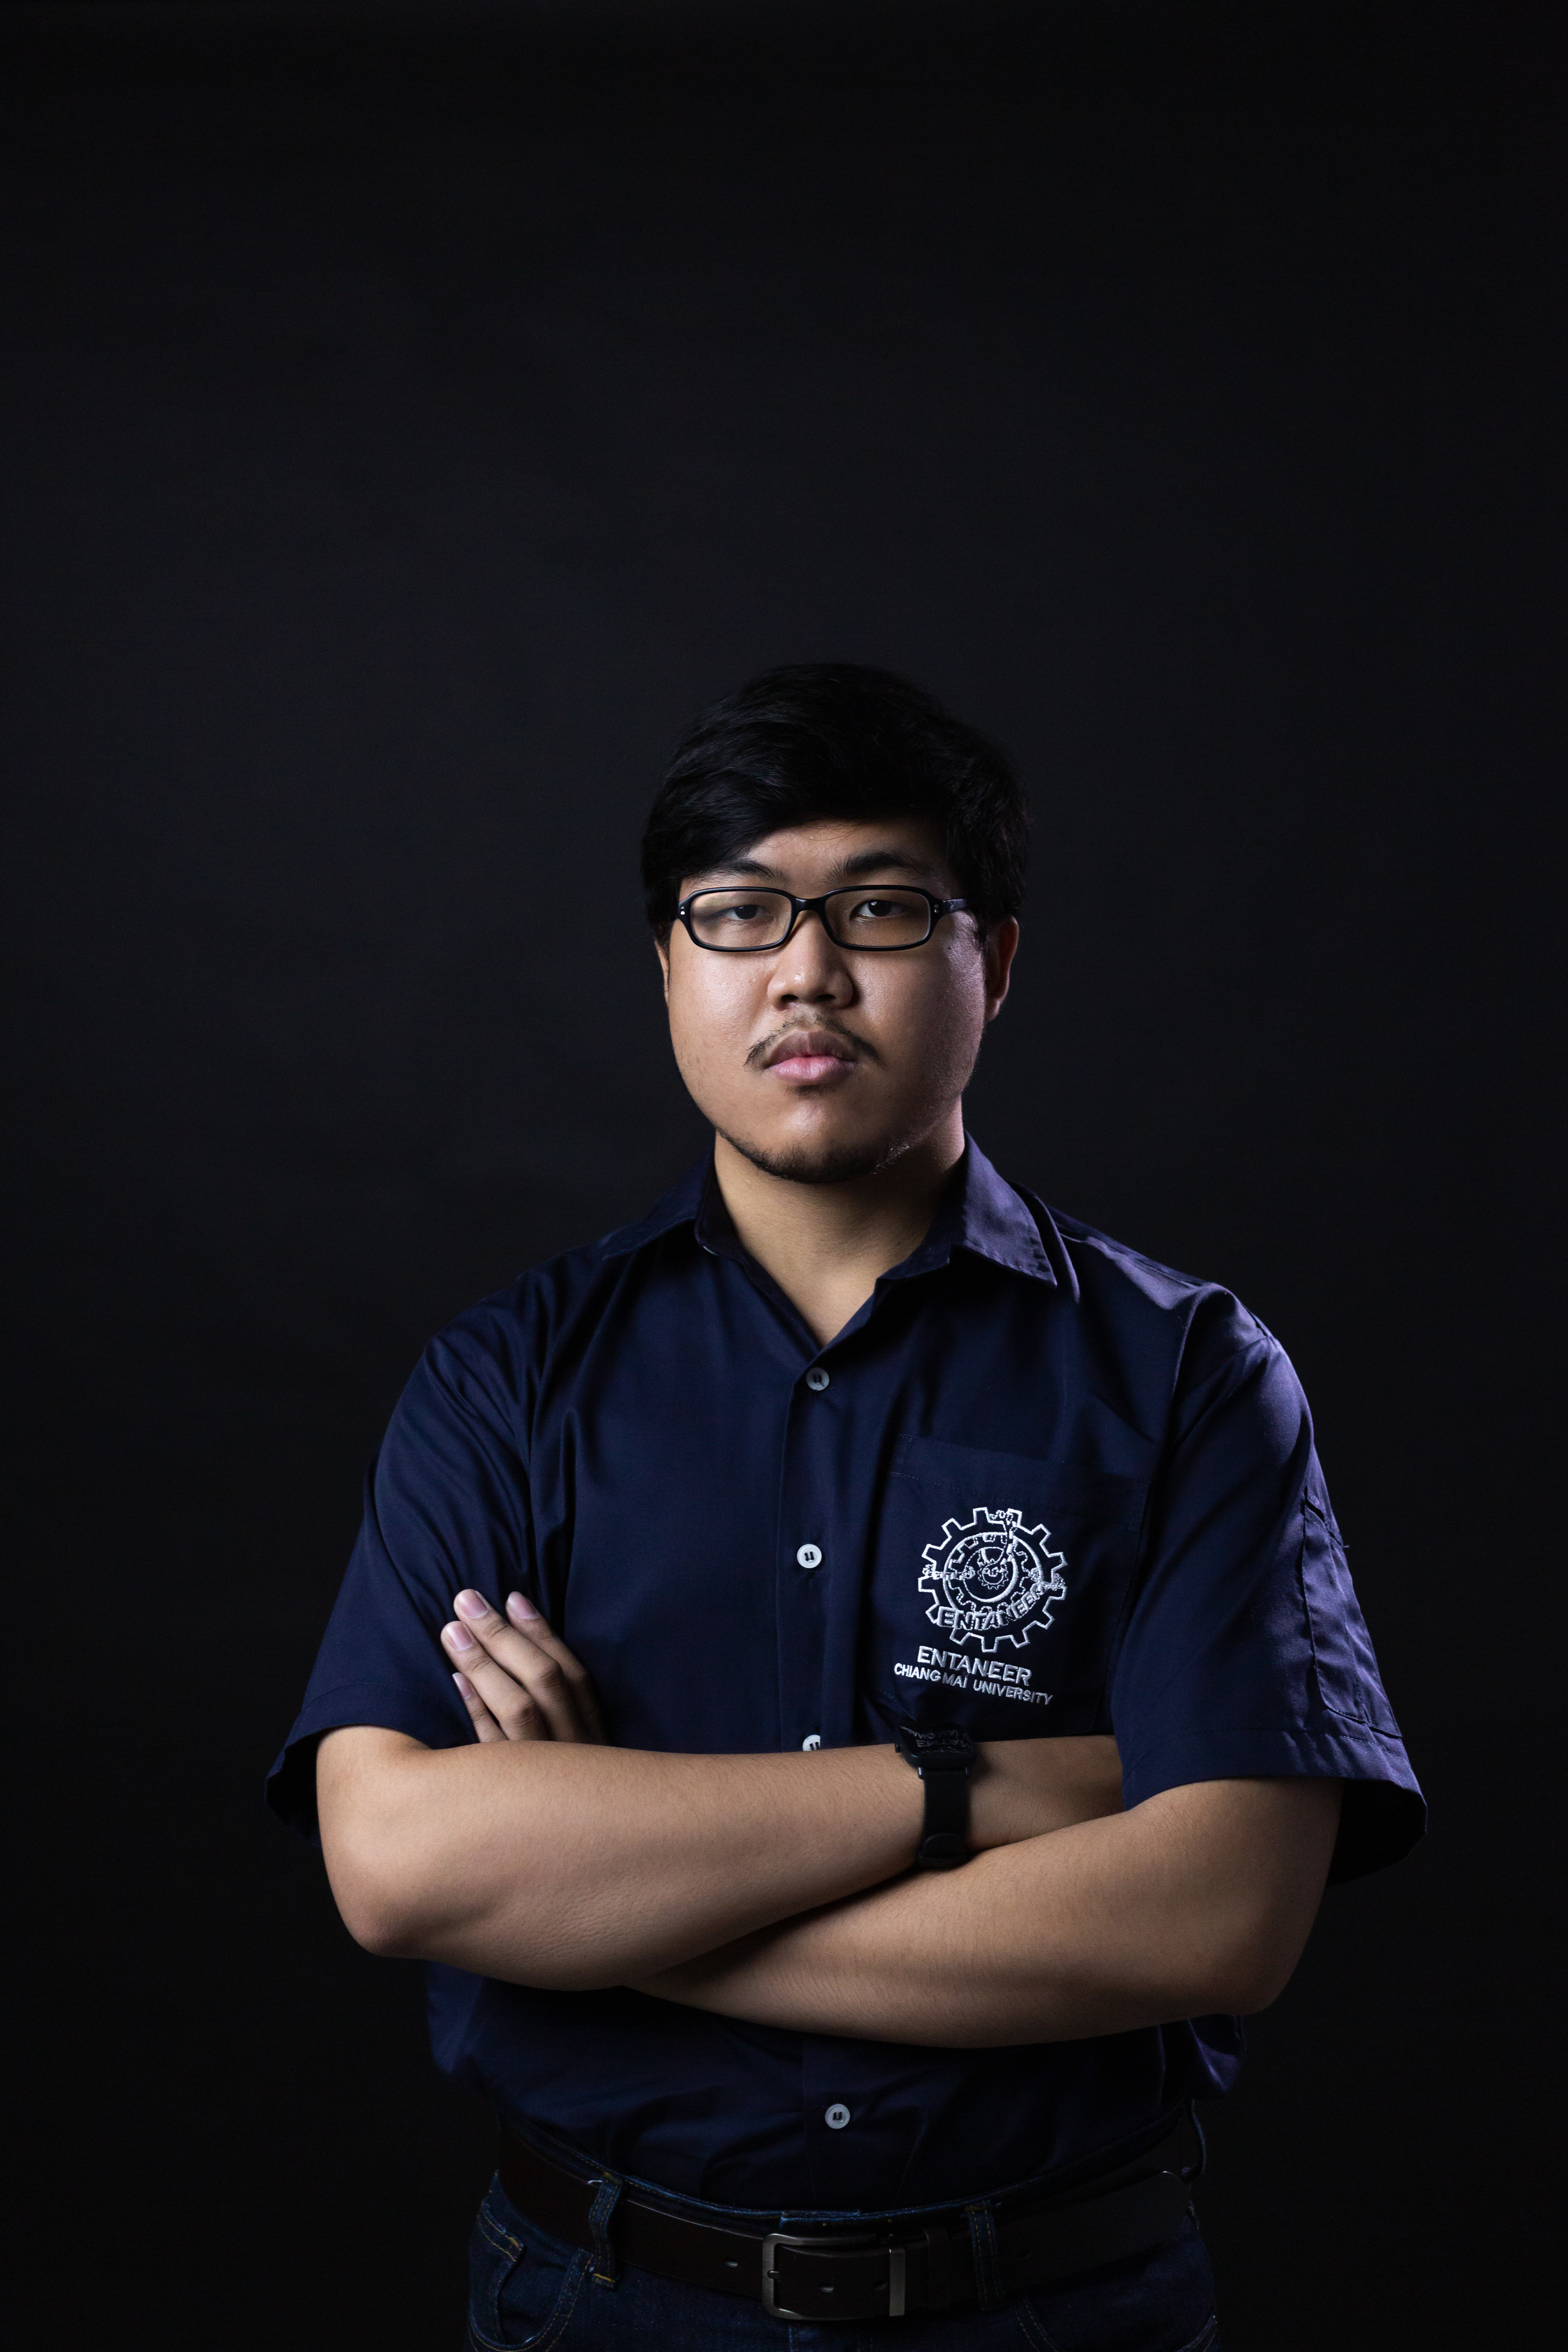
\includegraphics[width=1.5in]{image/SLP_0242.JPG}
\end{center}
นายธิษณ์ธนัย แก้วเพ็ชร์ เกิดเมื่อวันที่ 6 มิถุนายน พศ.2544 ณ จังหวัดเชียงใหม่ สําเร็จการศึกษาระดับ
มัธยมปลาย จาก โรงเรียนช่องฟ้าซินเซิงวาณิชบำรุง จังหวัดเชียงใหม่ เข้าศึกษาที่คณะวิศวกรรมศาสตร์ สาขาวิศวกรรมคอมพิวเตอร์ มหาวิทยาลัยเชียงใหม่ เมื่อเดือนมิถุนายน พ.ศ.2563
ก่อนจะเริ่มโครงงาน มีประสบการณ์ด้านพัฒนาเว็บแอปพลิเคชันฝั่ง front-end, Natural Language Processing และ human Computer Interaction
\end{biosketch}
\fi % \ifproject
\end{document}
